% -*- root: ../paper.tex -*-

While example data sets provide a good starting point for the \systemname knowledge-base, we anticipate that --- at least initially --- the training data will be too sparse to provide high quality matching suggestions.
To mitigate the effects of sparsity, \systemname relies on domain experts to curate its knowledge-base, refine existing matchers and define new matching heuristics.
This is intended to be an ongoing process, with incremental feedback from experts and users continuously refining the knowledge-base.
In this section we outline the design of an interface that streamlines knowledge-base refinement, starting from a knowledge-base trained on example data.
The central elements of this interface are 
(1) Visualizing the current quality of the knowledge base;
(2) Identifying problems with name/match-quality function pairs;
(3) Refining records in the knowledge base by removing or merging existing data, or adding expert knowledge.

\begin{figure}
	\centering
	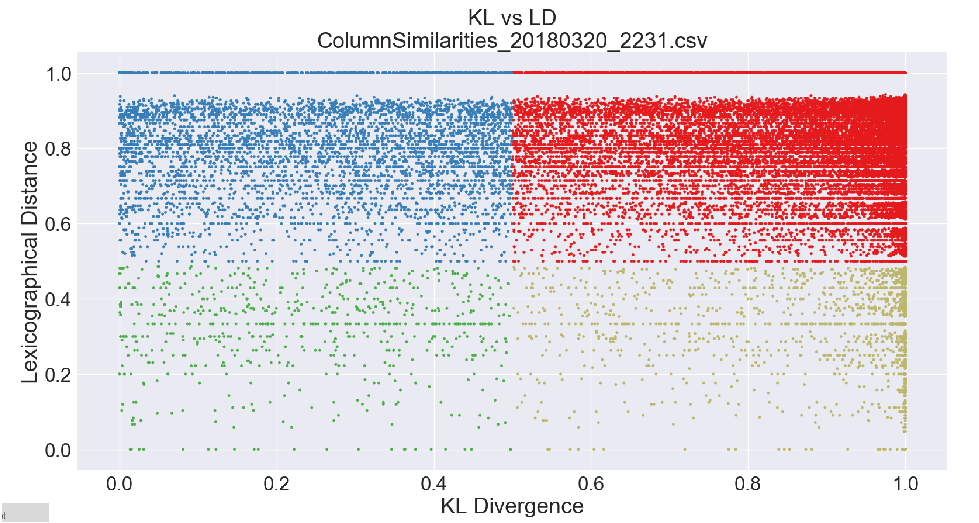
\includegraphics[width=1\columnwidth]{graphics/KBUI}
	\caption{Knowledge-base Editor: Showing Match Conflicts}
	\label{fig:editor:scatterplot}
	\trimfigurespacing
\end{figure}

\subsection{Refinement Interface}
The initial goal of the \systemname editor is to help domain experts quickly identify and resolve errors and redundancies in a preliminary knowlege-base freshly trained on new example data.  
The entry point into the refinement process is the \systemname editor's match-conflict explorer


\tinysection{Match Conflict Explorer}
This view, illustrated in Figure~\ref{fig:editor:scatterplot}, is a scatter plot with each point corresponding to one pair of concepts.
A point's x- and y-coordinates express, respectively, how different the concepts and their related matchers are.
In both cases, a value of 0 indicates that the concepts (resp., the corresponding matchers) are identical, while a value of 1 indicates that the concepts (matchers) are completely different.
We refer to these as concept- and match-differences.
In this preliminary version of the system, we define concept-difference to be the lowest Levenshtein distance between any two names associated with each of the concepts.
We define match difference as the lowest difference between any two matchers associated with a concept, with inter-matcher differences defined based on concept types.
For pairs of numerical distributions, this value is presently defined as the KL-Divergence between them.

The match conflict explorer helps identify overlapping or erroneous matchers, as well as duplicate or overlapping concepts.
Specifically, the view is divided into four quadrants.  The lower-left, shown in green indicates high concept-similarity and highly overlapping matchers (true positives).  
The upper-right, shown in red indicates the low concept-similarity and low matcher similarity (true negatives).
The upper-left, shown in blue identifies distinct concepts with similar matchers (potential false positives).  
The lower-right, shown in yellow identifies potentially similar concepts that have different matchers (potential false negatives).

\tinysection{Concept Pair View}
To resolve potential conflicts displayed in the explorer, users can select regions with a simple marquee tool or click on individual concepts (zoom is available if desired).
The selected concepts are displayed, along with their corresponding matchers as illustrated in Figure~\ref{fig:pairview}.

\begin{figure}
	\centering
	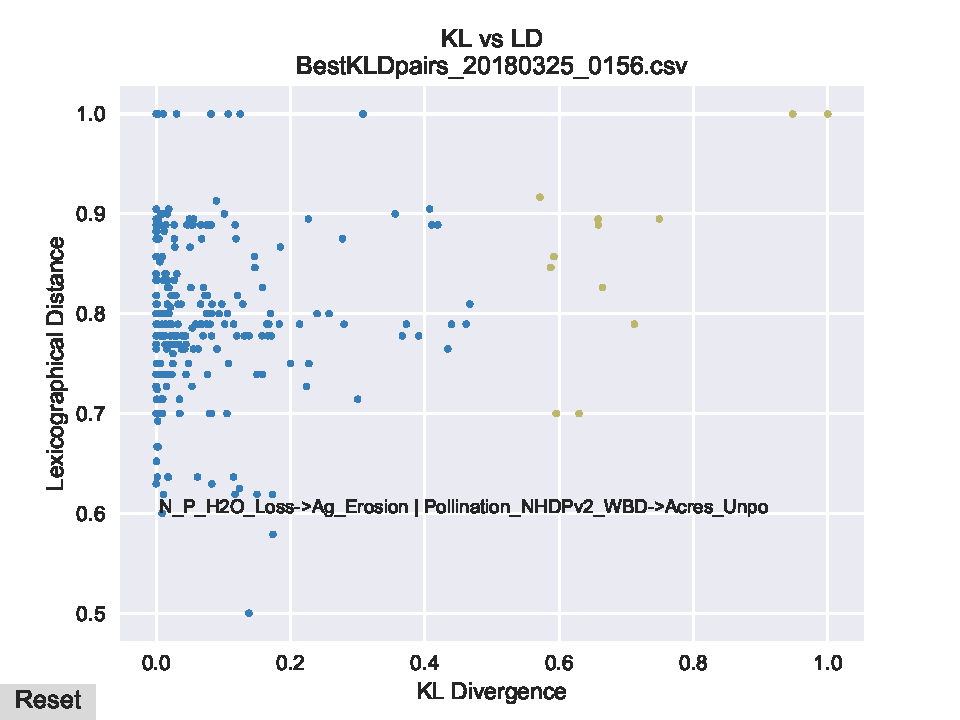
\includegraphics[trim={0 0 0 15mm},clip,width=\columnwidth]{graphics/Pair_view_data_callouts}
	\caption{Pair view in scatter plot}
	\label{fig:pairview}
	\trimfigurespacing
\end{figure}


% \begin{figure}
% \begin{tabular}{r|l}
% \textbf{How Y modifies X} & $(\namesymbol_x \oplus \namesymbol_y)(T_A)$ \\\hline
% X Or Y & $max(\namesymbol_x(T_A), \namesymbol_y(T_A))$\\
% X And Y & $\namesymbol_x(T_A) \cdot \namesymbol_y(T_A)$\\
% X Unless Y & $min(\namesymbol_x(T_A), \namesymbol_y(T_A))$\\
% Y Instead of X & $\namesymbol_y(T_A)$\\
% Y Suggests X & $1-(1-\namesymbol_x(T_A))(1-\namesymbol_y(T_A))$
% \end{tabular}
% \caption{Example augmentation modifiers}
% \label{fig:modifiers}
% \end{figure}

% \tinysection{Modifiers}
% Expert knowledge in the knowledge-base is encoded in two parts: 
% (1) A quality-match function that provides a heuristic encoding of the expert knowledge, and 
% (2) An augmentation modifier that indicates how the new quality match function is to be combined with the existing one.  
% Figure~\ref{fig:modifiers} illustrates several example modifiers together with intuitive phrasings of each.  
% For example, if the expert heuristic defines an unrelated approach to matching columns, the highest match value is used.


\subsection{Understanding Refinement in Practice}
As experts identify errors or redundancies in the knowledge-base, they will need to patch the knowledge-base accordingly.
To better understand their needs during this process, we selected 200 concept pairs at random from among the potential false-positives and potential false-negatives.
We inspected each pair of concepts selected in this way and determined a root cause for each.
We then grouped these root causes into seven categories.
The distributions of root causes of the potential false negatives and false positives are shown in Figures~\ref{fig:datatags:lowerright} and \ref{fig:datatags:upperleft}, respectively.
We now discuss each category in detail, along with an assessment of remedial actions available for resolving the potential error.

\begin{figure}
	\centering
	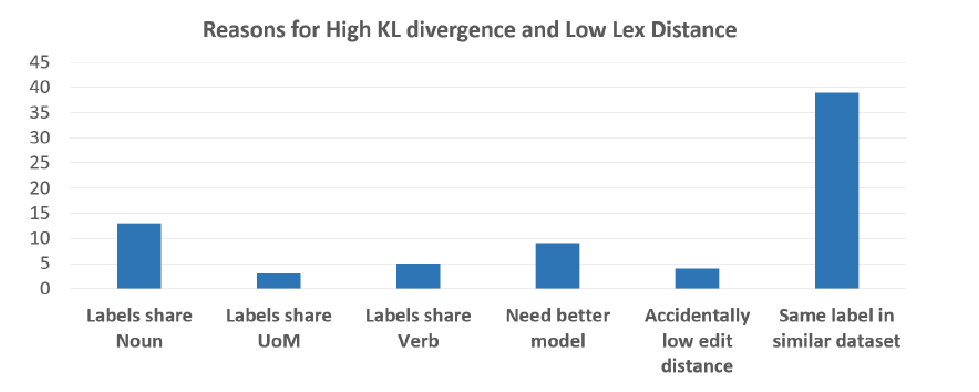
\includegraphics[width=\columnwidth]{graphics/Lower_right_quad}
	\caption{Root causes of potential false negatives.}
	\label{fig:datatags:lowerright}
	\trimfigurespacing
\end{figure}

\begin{figure}
	\centering
	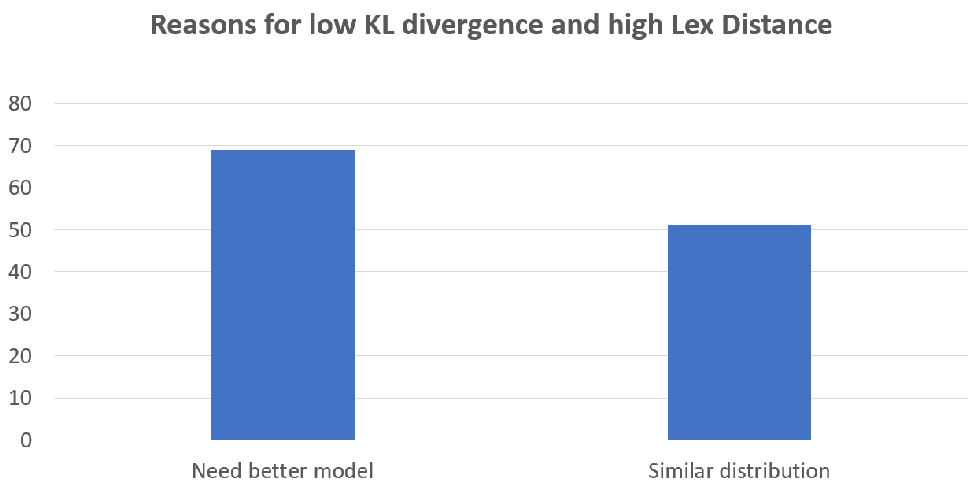
\includegraphics[width=\columnwidth]{graphics/Upper_left_quad}
	\caption{Root causes of potential false positives.}
	\label{fig:datatags:upperleft}
	\trimfigurespacing
\end{figure}

\smallskip
\subsubsection{Need a better model for training on examples}~\\
For 9 pairs in the lower right quadrant and 69 pairs in the upper left quadrant, the best fit matchers did not adequately describe the data distribution.
The training phase categorizes data by either uniform or normal distributions. 
However, we encountered distributions which can be described better using other distributions like zipfian or lognormal rather than normal or uniform.
Two examples are shown in Figure~\ref{fig:baddistributions}, following bimodal and zipfian distributions respectively, neither of which our preliminary implementation supported.

\textbf{Resolution}: Although a more robust learning process might address this issue (e.g., by supporting more standard distributions like lognormal or zipfian), the only way to truly address this issue definitively is to allow experts to manually define custom distributions (e.g., using splines).

\begin{figure}
	\centering
	\begin{subfigure}{0.49\columnwidth}
		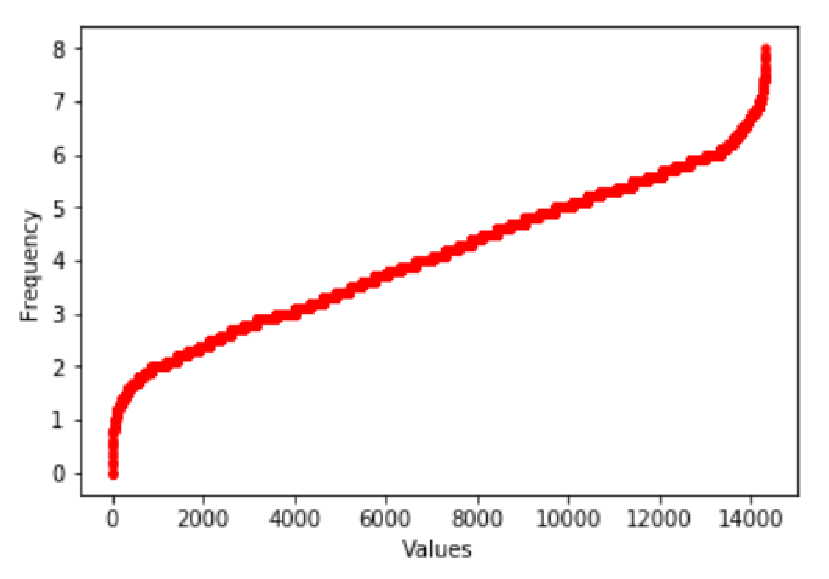
\includegraphics[width=1.1\textwidth]{graphics/Challenge1_1}
		\caption{\texttt{BIGGA\_AVG} (bimodal)}
		\label{fig:Distribution1}
	\end{subfigure}
	\begin{subfigure}{0.49\columnwidth}
		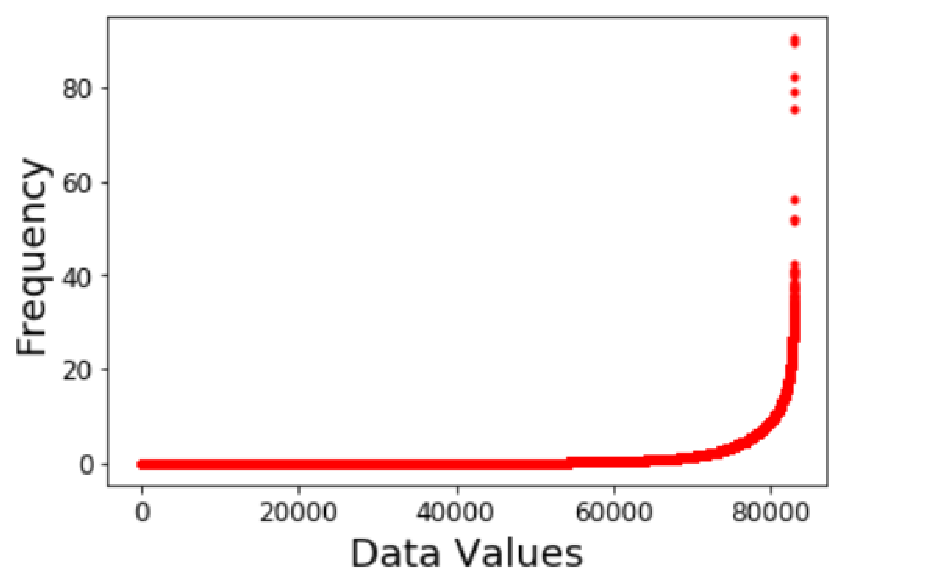
\includegraphics[width=1.1\textwidth]{graphics/Challenge7_1}
		\caption{\texttt{PctPasture\_slope9} (zipfian)}
		\label{fig:Distribution3}
	\end{subfigure}
	\trimfigurespacing
	\caption{Example CDFs of poorly fitted matchers}
	\label{fig:baddistributions}
	\trimfigurespacing
\end{figure}

% \begin{figure}[H]
% 	\centering
% 	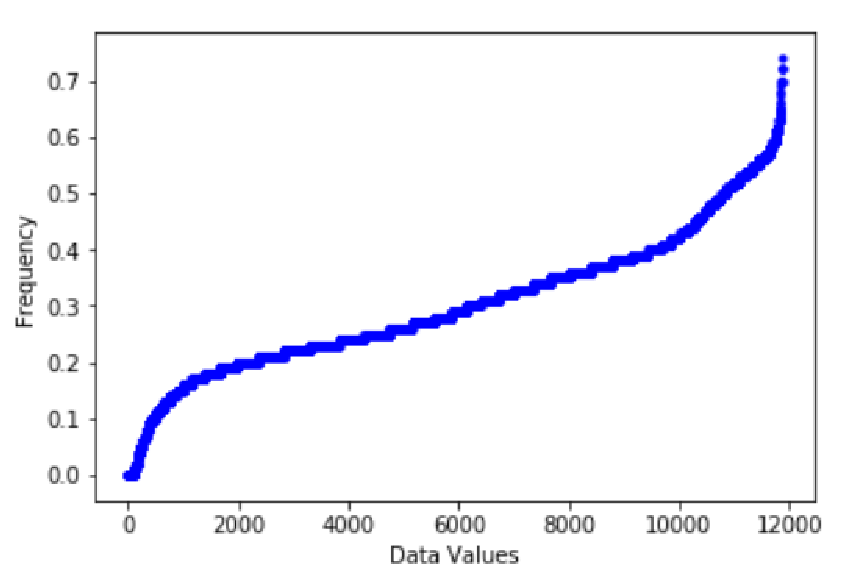
\includegraphics[width=0.8\columnwidth]{graphics/Challenge1_2}
% 	\caption{CDF of data distribution of column BIGGA\_AVG\_I}
% 	\label{fig:Distribution 2}
% \end{figure}

\smallskip
\subsubsection{Same column name in a different context}~\\
33 points, nearly half of the points sampled from among the potential false negatives, used the same name, but in different context.
For example, among the datasets used for this case study, we had two similar datasets in biodiversity domain. 
Both datasets consisted of data about flora and fauna, but from two different regions.

\textbf{Resolution}: Depending on context, a domain expert may wish to unify both concepts or keep them separate.
In the former case, the expert needs to be able to merge concept nodes in the knowledge-base together.  
In the latter case, the expert needs to be able to override the concept-difference to mark them as true negatives.

\smallskip
\subsubsection{Column names share measuring units, nouns, or verbs}~\\
In the case of 21 out of 79 potential false negatives, the limiting factor was our choice of similarity measure.
Common terminology not relevant to the meaning of the concept resulted in low lexical distances.
Specific examples we encountered were:
\begin{enumerate*}
\item Common measuring units like \texttt{FRUITHECTARES} or \texttt{VEGHECTARES} (3 pairs)
\item Common generic nouns like \texttt{BG\_Demand} or \texttt{MB\_Demand} (13 pairs)
\item Common verbs or statistical measures like \texttt{AVG}, \texttt{MEAN} or \texttt{MAX} (5 pairs).
\end{enumerate*}

\textbf{Resolution}:
As before, depending on context, a domain expert may wish to unify the underlying concepts (e.g., in the case of units like \texttt{HECTARES}), or not.
Similarly, this means that the expert needs to be able to merge concept nodes or override the concept difference measure.
However, in the case of this error, we can also pre-filter many of these cases by deleting common stop-words before computing the lexical distance (e.g., \texttt{AVG}).  

\smallskip
\subsubsection{Accidentally Levenshtein distance}~\\
In 4 remaining cases, the Levenshtein distance incorrectly identifies two column names as similar.  For example the column names \texttt{WTFL\_AVG} and \texttt{WET\_AG} are conceptually distinct, despite their low Levenshtein distances.

\textbf{Resolution}: 
This problem might be fixed by a more robust concept distance measure, such as one that relies on an ontology like YAGO~\cite{fabian2007yago}.  
However, any heuristic measure might still incorrectly label two distinct concepts as similar.  
Once again, the domain expert must be able to overide the concept-distance function.


\smallskip
\subsubsection{Distinct names with similar distributions.}~\\
Out of 120 points analyzed from the upper left quadrant, 51 had similar distributions.
Certain data distributions were incredibly common.
For example, there were (unsurprisingly) a large number of uniformly distributed integer values starting from 0: Index attributes.
These had often had distinct names.

\textbf{Resolution}:
As in many of the previous cases, based on context the expert may decide that this is a true positive, or may instead decide that the concepts are indeed distinct.
Similarly, the concepts may need to be merged, or not.
However, this case preseents one additional challenges: it indicates  matchers linked to distinct concepts that are liable to have similarly high match qualities on the same data --- conflicting matchers.
Hence, in both cases, the expert also needs to merge the conflicting matchers.

\smallskip
\subsubsection{True positives.}~\\
Although not the result of an actual problem, true positives indicate the presence of duplicate concepts, and consequently conflicting matchers.  As before, both the concepts and matchers need to be merged.


% \begin{figure}[H]
% 	\centering
% 	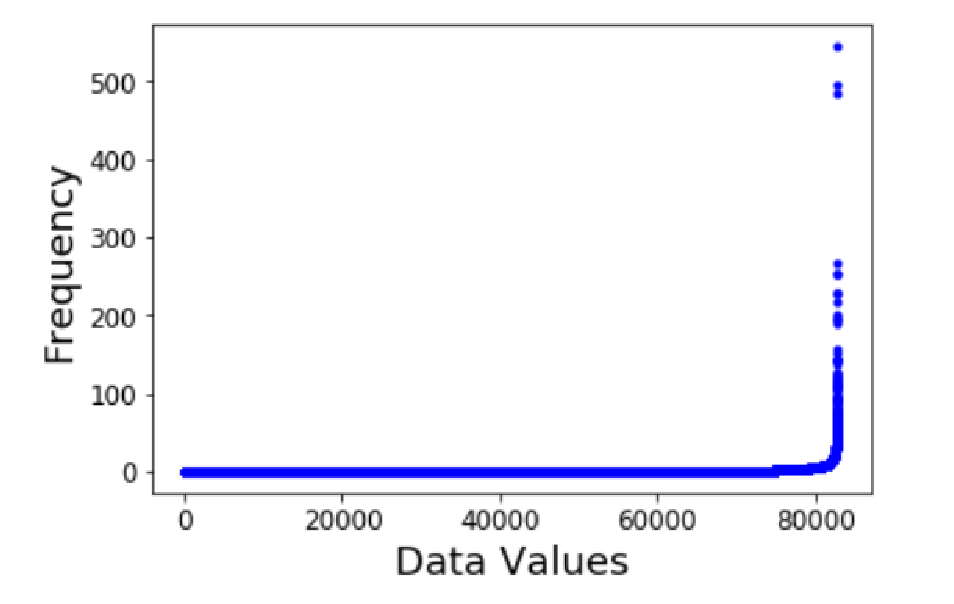
\includegraphics[width=0.8\columnwidth]{graphics/Challenge7_2}
% 	\caption{CDF of data distribution of column HistoricBuildings}
% 	\label{fig:Distribution 4}
% \end{figure}


\subsection{Editor Interface}
In addition to the match-conflict view, the \systemname editor provides a textual interface to search the knowledge-base for both concepts (by name), and matchers (by matcher-specific properties like the shape parameters of a distribution matcher).  
As previously noted, selecting pairs of concepts in the match-conflict view shows the pair of concepts and their associated matchers (as the result of a query).

Specifically, to resolve the data issues described above, the editor interface needs to allow experts to:
\begin{enumerate*}
	\item Manually define new data distributions, 
	\item Merge Concept Nodes, 
	\item Merge Match Nodes, and
	\item Override concept difference by forcing concepts to be distinct and defining stop-words
\end{enumerate*}


\tinysection{Editor Commands}
In addition to directly querying the knowledge-base, the editor provides commands for editing it:

\newcommand{\lokicommand}[2]{\smallskip\noindent \texttt{#1}: #2}

\lokicommand{EDIT [concept]}{
	Allows the expert to modify the names and matchers associated with a concept
}

\lokicommand{EDIT [matcher]}{
Allows the expert to modify the shape parameters and concepts of a matcher, as well as the matcher's default concept.
}

\lokicommand{MERGE [concept] [concept]}{
	Combines two concepts, creating a single concept by unioning their associated names and directing the associated matchers of both concepts to the same node.
}

\lokicommand{MERGE [matcher] OR [matcher]}{
	Instantiates a new matcher that emits the highest match quality detected by either matcher.  
	Concepts linked to the two matchers are migrated to the new matcher and the user is acked to pick one as a default for the new matcher.
}

\lokicommand{REPLACE [matcher] WITH [matcher]}{
	Deletes the former matcher and links the latter matcher to all of its concepts.  The latter matcher's default concept is preserved.
}



